\documentclass[10pt,mathserif]{beamer}

\input defs.tex

%\setbeamerfont*{frametitle}{size=\normalsize,series=\bfseries}

% from boyd
\mode<presentation>
{
\usetheme{default}
}
\setbeamertemplate{navigation symbols}{}
\usecolortheme[rgb={0.13,0.28,0.59}]{structure}
\setbeamertemplate{itemize subitem}{--}
\setbeamertemplate{frametitle} {
	\begin{center}
	  {\large\bf \insertframetitle}
	\end{center}
}

\newcommand\footlineon{
  \setbeamertemplate{footline} {
    \begin{beamercolorbox}[ht=2.5ex,dp=1.125ex,leftskip=.8cm,rightskip=.6cm]{structure}
      \footnotesize \insertsection
      \hfill
      {\insertframenumber}
    \end{beamercolorbox}
    \vskip 0.45cm
  }
}
\footlineon

\newcommand\blfootnote[1]{%
  \begingroup
  \renewcommand\thefootnote{}\footnote{#1}%
  \addtocounter{footnote}{-1}%
  \endgroup
}

\AtBeginSection[] 
{ 
	\begin{frame}<beamer> 
		\frametitle{Outline} 
		\tableofcontents[currentsection,currentsubsection] 
	\end{frame} 
}

%
\usepackage{animate}
\usepackage[export]{adjustbox}
\usepackage{centernot}
\usepackage{caption}
\usepackage{subcaption}
\usepackage{booktabs} % for professional tables
\usepackage{multirow}
\usepackage{microtype}
\usepackage{graphicx}
\usepackage{amsmath, amssymb, amsthm}
\usepackage{dsfont}
\usepackage{mathtools}
\usepackage{algorithm,algorithmic}
\usepackage{adjustbox}
% Setup TikZ
\usepackage{tikz}
\usepackage{tkz-graph}
\usepackage{pgfplots}
\usepackage{hyperref}

\usepackage[beamer]{hf-tikz} 
\usetikzlibrary{backgrounds,arrows,shapes.geometric,shapes.misc,positioning,patterns}


\tikzstyle{block}=[draw opacity=0.7,line width=1.4cm]

\renewcommand{\algorithmicrequire}{\textbf{initialize}}
\newcommand{\algorithmicinput}{\textbf{input}}
\newcommand{\algorithmicoutput}{\textbf{output}}
\newcommand{\INPUT}{\item[\algorithmicinput]}
\newcommand{\OUTPUT}{\item[\algorithmicoutput]}

\setbeamertemplate{theorems}[numbered]
\newtheorem{thm}{Theorem}
\newtheorem{defn}{Definition}
\newtheorem{prop}{Proposition}

% Author, Title, etc.
\title{Learning Discrete and Continuous Factors of Data via Alternating Disentanglement}
\author{author}
\institute
    {Seoul National University}
\date{2017.09.01}

% hide solutions in handout mode
\newcommand\hideit[1]{%
  \only<0| handout:1>{\mbox{}}%
  \invisible<0| handout:1>{#1}}

% independence symbol
\newcommand{\indep}{\raisebox{0.05em}{\rotatebox[origin=c]{90}{$\models$}}}
\tikzset{above left offset={0.0,0.6},below right offset={0.0,-0.5}}

% The main document
\begin{document}
\begin{frame}
  \titlepage
\end{frame}

\section{Intro}
\setbeamercolor{block body}{parent=normal text,use=block title,bg=block title.bg!15!bg}
\setbeamercolor{block title}{use=structure,fg=white,bg=structure.fg!75!black}

\begin{frame}
\frametitle{Disentanglement}
\begin{figure}
\centering
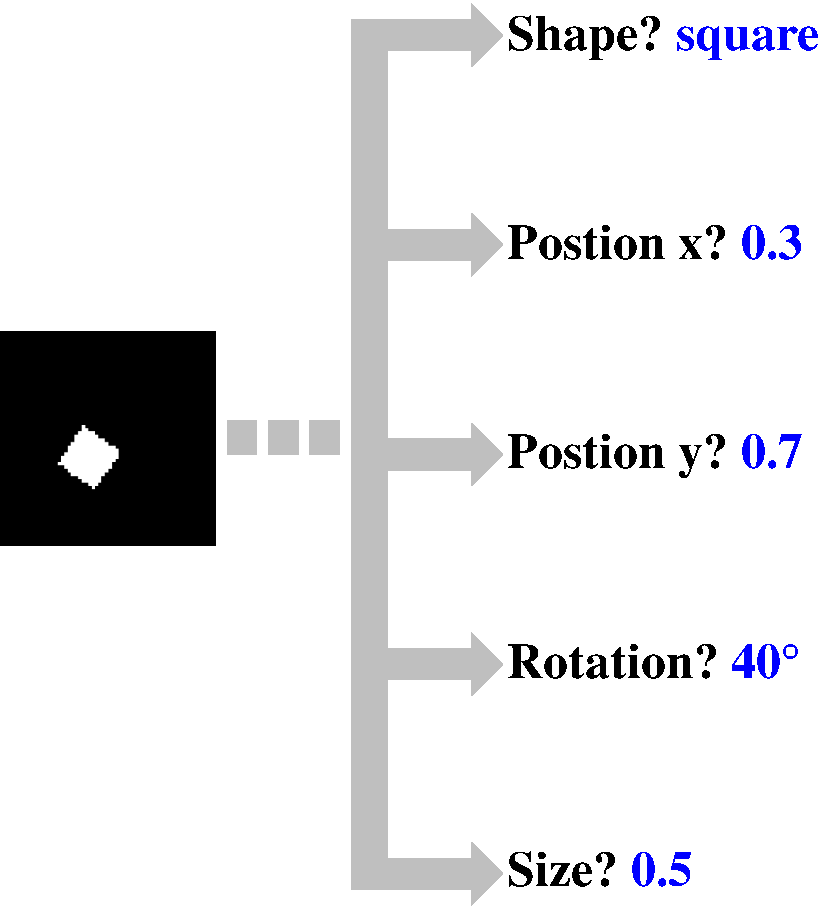
\includegraphics[width=0.6\linewidth]{disentanglement}
\end{figure}
\end{frame}

\begin{frame}
\frametitle{Motivation}

\begin{figure}
\centering
\only<1>{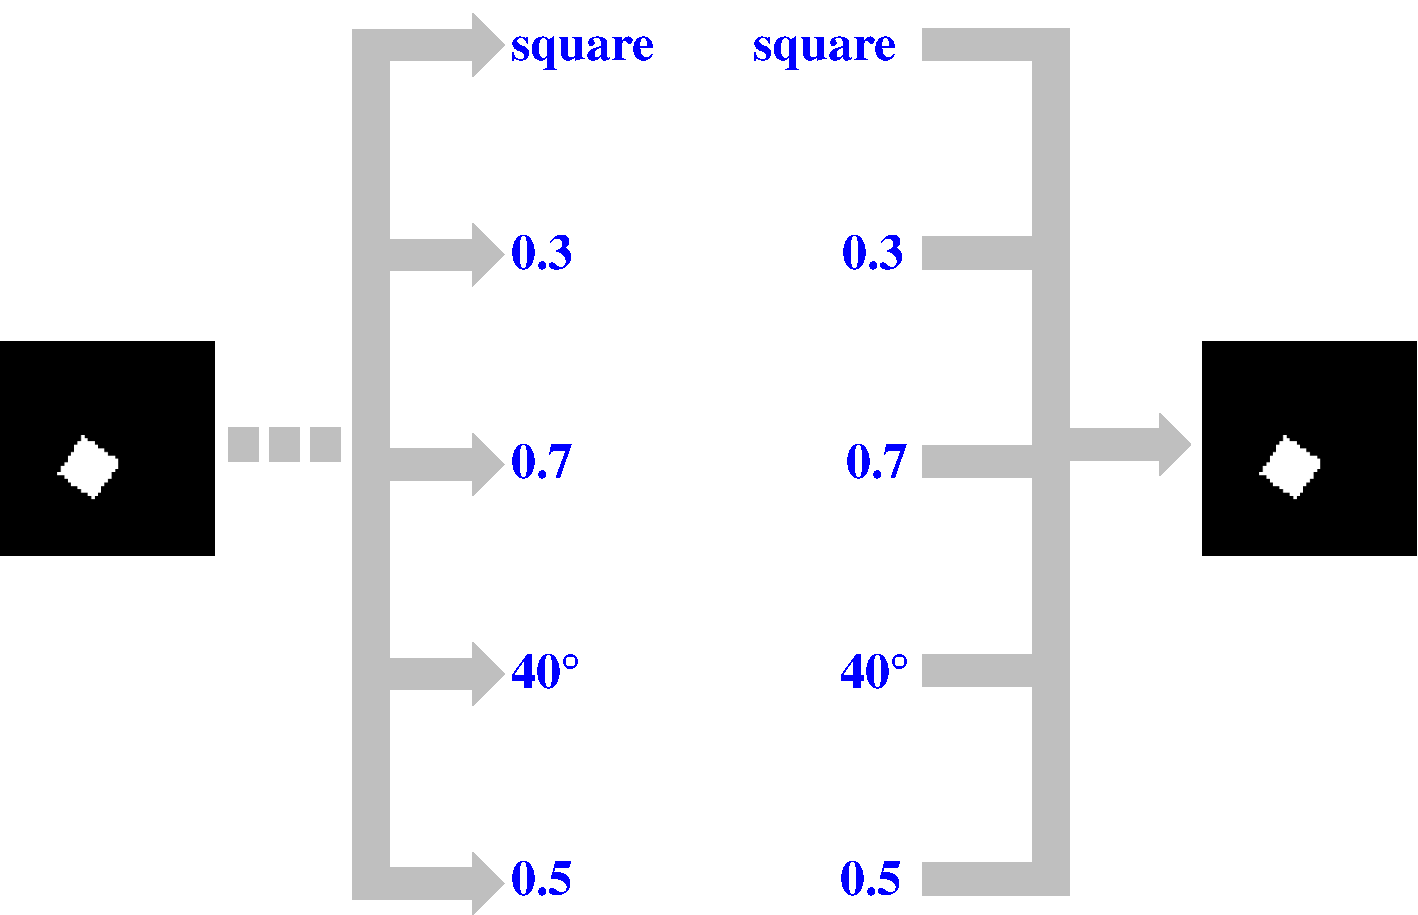
\includegraphics[page=1, width=\linewidth]{motivation}}%
\only<2>{\includegraphics[page=2, width=\linewidth]{motivation}}%
\only<3>{\includegraphics[page=3, width=\linewidth]{motivation}}%
\only<4>{\includegraphics[page=4, width=\linewidth]{motivation}}%
\only<5>{\includegraphics[page=5, width=\linewidth]{motivation}}%
\only<6>{\includegraphics[page=6, width=\linewidth]{motivation}}%
\only<7>{\includegraphics[page=7, width=\linewidth]{motivation}}%
\end{figure}
\end{frame}

\begin{frame}
\frametitle{Motivation}
\begin{itemize}\itemsep=20pt
\item Our interest is to {\color{blue}{disentangle}} the underlying explanatory factors of data {\color{blue}{without any supervision.}}\pause
\item We require a stable disentanglement framework to capture {\color{blue}{continuous}} and {\color{blue}{discrete}} factors.
%%\pause\item {\color{blue}{VAE}} framework guarantees a stable framework compared to GAN framework.
\end{itemize}
\end{frame}

\begin{frame}
\frametitle{Contributions}
\begin{itemize}\itemsep=20pt
        \item We propose a simple procedure for penalizing the {\color{blue}{total correlation}} without any extra {\color{blue}{discriminator network(FactorVAE)}}\footnote{{\color{blue}{Kim, H. and Mnih, A.}} Disentangling by factorising. {\color{gray}{ICML2018}}} or {\color{blue}{importance sampling}} \footnote{{\color{blue}{Chen, T. Q., Li, X., Grosse, R. B., and Duvenaud, D. K.}} Isolating sources of disentanglement in variational autoencoders. {\color{gray}{NIPS2018}}} in the {\color{blue}{$\beta$-VAE}} \footnote{{\color{blue}{Higgins, I., Matthey, L., Pal, A., Burgess, C., Glorot, X., Botvinick, M., Mohamed, S., and Lerchner, A.}} beta-vae: Learning basic visual concepts with a constrained variational framework. {\color{gray}{ICLR2017}}} framework.\pause
\item We propose an {\color{blue}{alternating disentanglement method}} to disentangle discrete and continuous factors without lumping both the continuous and discrete factors into a single latent vector.
\end{itemize}
\end{frame}

\section{Method}
\begin{frame}
\frametitle{$\beta$-VAE framework}
\begin{itemize}\itemsep=20pt
\item VAE is a latent variable model that pairs a top-down decoding generator ($\theta$) and a bottom-up encoding inference network ($\phi$).\pause
%%\item A variational lower bound of the marginal log-likelihood, $\mathbb{E}_{x \sim p(x)} \log p(x)$, is maximized.\pause
\item VAE objective or the variational lower bound is,
\begin{align}
\mathcal{L}(\theta,\phi) = \mathbb{E}_{x \sim p(x)} \big[&\mathbb{E}_{z \sim q_\phi(z \mid x)} \log p_\theta(x \mid z)- \beta D_\text{KL}\left(q_\phi(z \mid x) \parallel p(z)\right)\big],\nonumber
\end{align}
where $p(z)$ is the fully factorized standard normal prior.
%%\item Maximizing the objective can be viewed as maximizing the lower bound on the mutual information between the data $x$ and the latent code $z$ with the KL term.
%%\begin{align}
%%    I(x;z) - \beta \mathbb{E}_{x\sim p(x)}D_\text{KL}(q_\phi(z\mid x) \parallel p(z)) \nonumber
%%\end{align}
\end{itemize}
\end{frame}

\begin{frame}
\frametitle{$\beta$-VAE framework}
\begin{itemize}\itemsep=12pt
\item We can decompose KL regularizer term. Concretely,
\begin{align}
&\mathbb{E}_{x \sim p(x)} D_\text{KL}(q(z| x) ~||~ p(z))\nonumber \\
&~~~=I(x;z) + \underbrace{D_\text{KL}(q(z) \parallel \prod_j q(z_j))}_{=~\text{Total correlation},~ TC(z)} + \sum_j D_\text{KL}(q(z_j) \parallel p(z_j)),\nonumber
\end{align}
        where $q(z)(=\mathbb{E}_{p(x)}[q(z\!\mid\!x)])$ denotes the marginal posterior. 
\end{itemize}
\end{frame}

\begin{frame}
\frametitle{Total Correlation $TC(z)$}
\begin{itemize}\itemsep=20pt
\item Total correlation or $TC(z)$ is a popular measure quantifying the redundancy among a set of $m$ random variables. \pause
\item Multivariate version of mutual information $I(\cdot, \cdot)$
\begin{align}
I(z_1,z_2)= D_\text{KL}(q(z_1,z_2) \parallel q(z_1)q(z_2))=TC(z_{1:2})\nonumber
\end{align}
        \vspace{-2em}
\pause \item {\color{blue}{Penalizing TC}} leads the model to learn {\color{blue}{statistically independent factors}} in the data which is a crucial component in disentangled representations. 
%%\begin{align}
%%TC(z) = D_\text{KL}(q(z) \parallel \prod_j q(z_j)),\nonumber
%%\end{align}
\end{itemize}
\end{frame}

\begin{frame}
\frametitle{Limitation of $\beta$-VAE}
\begin{itemize}\itemsep=20pt
\item $\beta$-VAE objective is
\begin{align}
\mathbb{E}_{x \sim p(x)} \big[\mathbb{E}_{z \sim q_\phi(z \mid x)} \log p_\theta(x \mid z)- \beta D_\text{KL}\left(q_\phi(z \mid x) \parallel p(z)\right)\big].\nonumber
\end{align}
\item $\beta$-VAE sets $\beta > 1$ to penalize $TC(z)$ which leads to statistically independent and disentangled representations. \pause
\item However, it penalizes the mutual information($=I(x,z)$) between the data and the latent variables. 
%%    \footnote{
%%\begin{align}
%%&\mathbb{E}_{x \sim p(x)} D_\text{KL}(q(z| x) ~||~ p(z))\nonumber \\
%%&~~~=I(x;z) + \underbrace{D_\text{KL}(q(z) \parallel \prod_j q(z_j))}_{=~\text{Total correlation},~ TC(z)} + \sum_j D_\text{KL}(q(z_j) \parallel p(z_j)),\nonumber
%%\end{align}}
\end{itemize}
\end{frame}

\begin{frame}
\frametitle{Overview of our method}
\begin{figure}
\includegraphics[page=2, width=\linewidth]{arch}
\end{figure}
\end{frame} 

\begin{frame}
\frametitle{Our method}
\begin{prop}
The mutual information between a single random variable and the rest can be factorized as
\[I(z_{1:i-1}; z_i) = TC(z_{1:i}) - TC(z_{1:i-1})\]
\end{prop}
\begin{prop}
The mutual information between $x$ and partitions of $z = [z_1, z_2]$ can be factorized as,
\[I(x; [z_1, z_2]) = I(x;z_1) + I(x; z_2) - I(z_1; z_2)\]
\end{prop}
\end{frame}

\begin{frame}
\frametitle{Our method}
\begin{itemize}\itemsep=12pt
\item By proposition1,
\begin{align}
TC(z)&=\underbrace{TC(z_{1:2})}_{= I(z_1; z_2)} + \sum_{i=3}^m \left( \underbrace{TC(z_{1:i}) - TC(z_{1:i-1})}_{= I(z_{1:i-1}; z_i)} \right)\nonumber\\
&= \sum_{i=2}^m I(z_{1:i-1}; z_i).\nonumber
\end{align}
\pause
\item We aim at penalizing $TC(z)$ by sequentially penalizing the individual summand $I(z_{1:i-1};z_i)$.
\end{itemize}
\end{frame}

\begin{frame}
\frametitle{Our method}
\begin{itemize}\itemsep=20pt
\item By proposition2,
\begin{align}
&I(x;z_{1:i}) = I(x;z_{1:i-1}) + I(x;z_{i}) - I(z_{1:i-1};z_{i}).\nonumber\\
&~~~~\onslide<2->{\uparrow} \only<1>{\qquad\qquad\quad\uparrow} \onslide<2->{\qquad\qquad\quad\bullet\quad\qquad\qquad\uparrow\qquad\qquad\quad\downarrow}\nonumber
\end{align}
\item This factorization motivates a maximization algorithm sequentially updating the left hand side $I(x; z_{1:i})$ for all $i=2,\ldots,m$ which in turn minimizes each summand, $\mathbf{I(z_{i-1};z_i)}$.
\onslide<3->{\item Sequentially, we maximize $I(x;z_{1:i})$ by penalizing $z_{i+1:m}$ with high $\beta$($\beta_h$) and the others with small $\beta$($\beta_l$).}
\end{itemize}
\end{frame}

\begin{frame}
\frametitle{Our method}
\begin{figure}
\only<1>{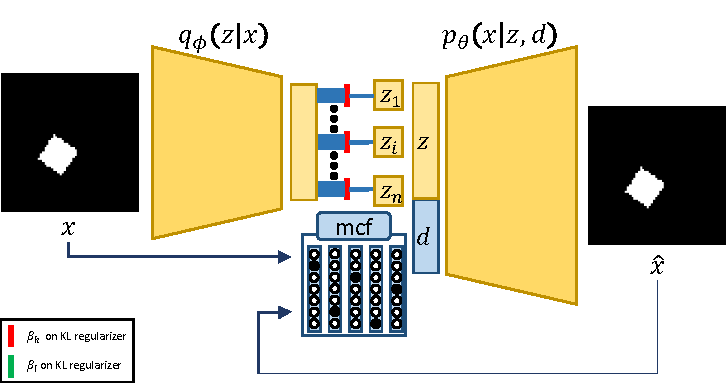
\includegraphics[page=1, width=\linewidth]{arch}}%
\only<2>{\includegraphics[page=2, width=\linewidth]{arch}}%
\only<3>{\includegraphics[page=3, width=\linewidth]{arch}}%
\only<4>{\includegraphics[page=4, width=\linewidth]{arch}}%
\end{figure}
\begin{itemize}
\item Every latent dimensions are heavily penalized with $\beta_h$. Each penalty on latent dimension is sequentially relieved one at a time with $\beta_l$ in a cascading fashion.
\end{itemize}
\end{frame} 

\begin{frame}
\frametitle{Graphical model}
\begin{figure}[bp]
\centering
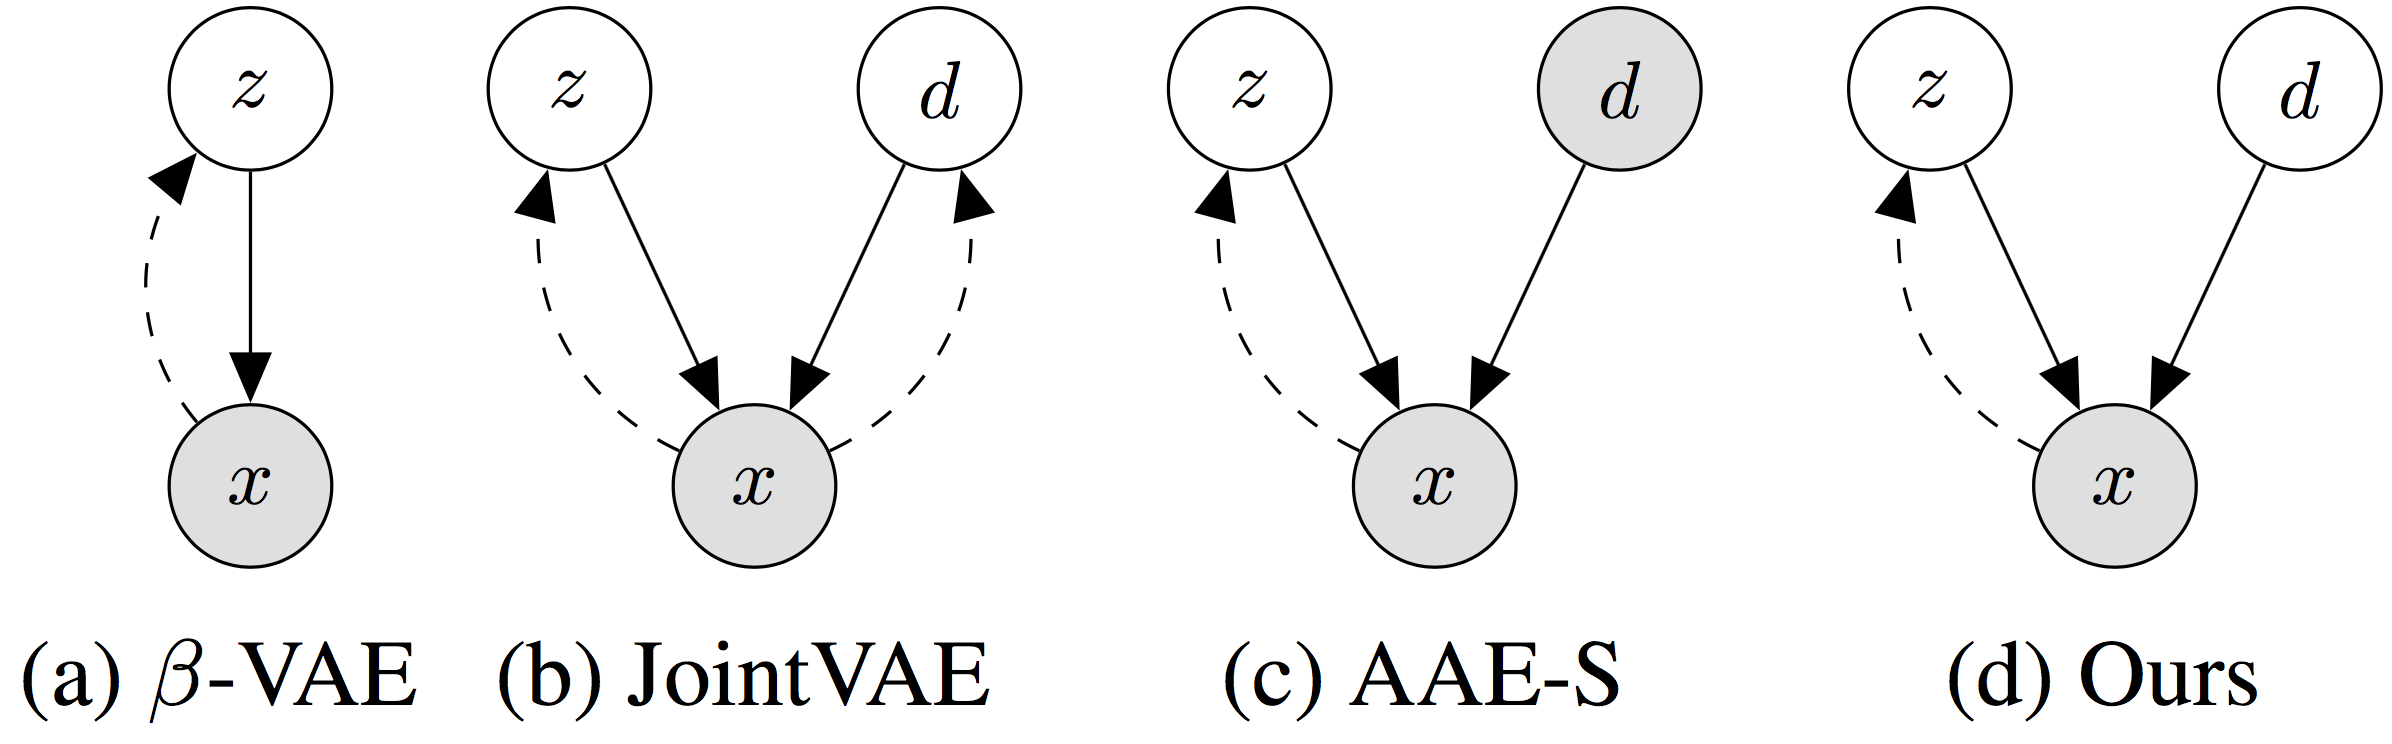
\includegraphics[width=1.0\linewidth]{graphical_model.png}
    \caption{Graphical models view of $\beta$-VAE, JointVAE, AAE with supervised discrete variables(AAE-S), and our method. Solid lines denote the generative process and the dashed lines denote the inference process. $x,z,d$ denotes the data, continuous latent code, and the discrete latent code respectively.}
\end{figure}
\end{frame} 

\begin{frame}
\frametitle{Joint distribution}
\begin{itemize}
\item JointVAE
\begin{align}
    q(z,x,d) = p(x)q(z,d|x)\nonumber
\end{align}
\item AAE-S
\begin{align}
    q(z,x,d) = \begin{cases}p(x)q(z|x) & \text{if $d=y$} \\ 0 & \text{otherwise}\end{cases},\nonumber
\end{align}where $y$ is a provided ground truth discrete factors through supervision.
\item CascadeVAE
\begin{align}
    q(z,x,d) = \begin{cases}p(x)q(z|x) & \text{if $d = \argmax_{\hat{d}} p(x|z,\hat{d})$} \\0 &\text{otherwise}\end{cases}\nonumber
\end{align}
\end{itemize}
\end{frame}

\begin{frame}
\frametitle{Drawbacks of JointVAE}
\begin{itemize}\itemsep=12pt
\item 
\begin{align}
    q(z,x,d) = p(x)q(z,d|x)\nonumber
\end{align}
\item JointVAE can be viewed as  augmenting the continuous latent variables with discrete latent variables ($z=[z'; d]$) in the $\beta$-VAE framework.\pause
\item However, simply lumping the latent variables together offloads the entire burden of jointly modeling both the continuous and discrete factors to the variational posterior which can be very challenging.
\end{itemize}
\end{frame} 

\begin{frame}
\frametitle{AAE-S}
\begin{itemize}\itemsep=12pt
\item
\begin{align}
    q(z,x,d) = \begin{cases}p(x)q(z|x) & \text{if $d=y$} \\ 0 & \text{otherwise}\end{cases},\nonumber
\end{align}where $y$ is a provided ground truth discrete factors through supervision.
\item AAE have investigated learning continuous latent representations while providing the discrete factors through supervision(e.g. class labels in MNIST).\pause
\item Model can learn drastically better continuous representations when the burden of simultaneously modeling the continuous and discrete factors is relieved.
\end{itemize}
\end{frame} 

\begin{frame}
\frametitle{Our method}
\begin{itemize}\itemsep=12pt
\item
\begin{align}
    q(z,x,d) = \begin{cases}p(x)q(z|x) & \text{if $d = \argmax_{\hat{d}} p(x|z,\hat{d})$} \\0 &\text{otherwise}\end{cases}\nonumber
\end{align}
\item Inspired by these findings, our idea is to alternate between finding the most likely discrete configuration of the variables given the continuous factors, and updating the parameters ($\phi,\theta$) given the discrete configurations. 
\end{itemize}
\end{frame} 

\begin{frame}
\frametitle{Alternating minimization scheme}
    \begin{itemize}
\item Our goal is to maximize the variational lower bound of the following objective,
\small
\begin{align}
&\mathcal{L}(\theta,\phi)=I(x; [z,d]) - \beta \mathbb{E}_{x\sim p(x)} D_\text{KL}(q_\phi(z \mid x) \parallel p(z))-\lambda D_\text{KL} (q(d) \parallel p(d))\nonumber\\
& \geq H(x)+\int \sum_d q(x,z,d) \log q_{\theta, \phi}(x|z,d) dz dx\nonumber\\
&~~-\beta \mathbb{E}_{x\sim p(x)} D_\text{KL}(q_\phi(z \mid x) \parallel p(z)) - \lambda D_\text{KL} (q(d) \parallel p(d))\nonumber\\
&\geq H(x)+\mathbb{E}_{x\sim p(x)}[\mathbb{E}_{z,d\sim q_{\phi, \theta}(\cdot | x)}[\log p_{\theta}(x|z,d)]]\nonumber\\
&\quad-\beta \mathbb{E}_{x\sim p(x)} D_\text{KL}(q_\phi(z \mid x) \parallel p(z))- \lambda (S\mathbb{E}_{d, d' \sim q(d)}[\mathds{1}(d=d')]-1).\nonumber
\end{align}
    \end{itemize}
\end{frame}

\begin{frame}
\frametitle{Alternating minimization scheme}
\begin{itemize}\itemsep=12pt
\item Note the lower bound has an inner maximization step over the discrete factors embedded in the variational posterior.
\item Data is sampled $x^{(i)} \in \mathcal{X}, i=1, \ldots, n$.
\item The continuous latent variables($z^{(i)}$) are samples from the decoder $q_\phi(\cdot \mid x^{(i)})$. 
\item The discrete latent variables are represented using one-hot encodings of each variables $d^{(i)} \in \{e_1, \ldots, e_S\}$.
\end{itemize}
\end{frame}

\begin{frame}
\frametitle{Alternating minimization scheme}
\begin{itemize}
\item
    After rearranging the terms, we arrive at the following optimization problem.
\begin{align}
\label{eqn:master_eqn}
&\maximize_{\theta, \phi} \left(\underbrace{\maximize_{d^{(1)},\ldots d^{(n)}} \sum_{i=1}^n {u_\theta^{(i)}}^\intercal d^{(i)} - \lambda' \sum_{i\neq j} {d^{(i)}}^\intercal d^{(j)}}_{:= \mathcal{L}_{LB}(\theta, \phi)} \right)\nonumber\\
&\qquad\qquad\quad - \beta \sum_{i=1}^n D_{KL}(q_\phi(z|x^{(i)})||p(z))\nonumber\\
&\text{\ \  subject to }~~ \| d^{(i)} \|_1 = 1,~ d^{(i)} \in \{0,1\}^S,~ \forall i, \nonumber
\end{align}
where $u_\theta^{(i)}$ denotes the vector of the  likelihood $\log p_\theta(x^{(i)}|z^{(i)}, e_k)$ evaluated at each $k \in [S]$.
        
\end{itemize}
\end{frame}

\begin{frame}
\frametitle{Alternating minimization scheme}
\begin{itemize}
    \item The inner maximization problem $\mathcal{L}_{LB}(\theta, \phi)$  over the discrete variables $[d^{(1)},\ldots,d^{(n)}]$ subject to the sparsity equality constraints can be exactly solved in polynomial time via \emph{minimum cost flow}(mcf) without  continuous relaxation \footnote{ {\color{blue}{Jeong, Y. and Song, H. O.}} Efficient end-to-end learning for quantizable representations. {\color{gray}{ICML2018}} }. 
\end{itemize}
\end{frame}


\section{Experiments}
\begin{frame}
\frametitle{Pseudocode}
\begin{algorithm}[H]
\caption{CascadeVAE}
\footnotesize
\begin{algorithmic}[1]
\INPUT Data $\{x^{(i)}\}_{i=1}^N$, Encoder($q_\phi$), Decoder($p_\theta$), $\beta_l, \beta_h$, $r, t_d$, optimizer $g$
\STATE Initialize parameters $\phi, \theta$.
\STATE Set $\beta_j=\beta_h,~$ $\forall j$ and $d^{(i)}=0,$ $~~\forall i\in [N]$
\STATE Set $j=1$.
\FOR{$t=1,\ldots,$MAXITER}
\STATE \textbf{if} $t$ is a multiple of $r$
\STATE $~~~$Switch $\beta_j$ to $\beta_l$ and $j\leftarrow j+1$
\STATE Randomly select batch $\{x^{(i)}\}_{i \in \mathcal{B}}$
\STATE Sample $z^{(i)}_\phi \sim q_{\phi}(z|x^{(i)})$ $\forall i \in \mathcal{B}$ 
\STATE \textbf{if} $t>t_d$
\STATE $~~~$ Update $u_\theta^{(i)}$ by computing $\log p_\theta(x^{(i)}|z^{(i)}, e_k)$ $\forall k$
\STATE $~~~$ Compute $\mathcal{L}_{LB}(\theta, \phi)$ by solving for the optimal \\
\qquad assignment $\{d^{(i)}\}_{i\in \mathcal{B}}$ via minimum cost flow 
\STATE $\theta, \phi \leftarrow g\left(\nabla_{\theta,\phi} \mathcal{L}_{LB}(\theta,\phi)\right)$
\ENDFOR
\end{algorithmic}
\end{algorithm}
\end{frame}


\begin{frame}
\frametitle{Notation}
\begin{itemize}\itemsep=12pt
\item We denote our method without the discrete variables as \textbf{CascadeVAE-C}.
\item We denote our full method as \textbf{CascadeVAE}. 
\item We evaluate with disentanglement score introduced in \textbf{FactorVAE} and unsupervised classification accuracy.
\item Baselines are \textbf{$\beta$-VAE, JointVAE, FactorVAE}
\end{itemize}
\end{frame}

\begin{frame}
\frametitle{dSprites Dataset}
\begin{itemize}\itemsep=20pt
\item This dataset is used to assess the disentanglement properties of unsupervised learning methods.\pause
\item There are 6 ground truth independent latent factors\\
    (e.g. color, shape, scale, orientation, position x, position y).\pause
\item There are $737280(=1\times3\times6\times40\times32\times32)$ images.
\end{itemize}
\end{frame}

\begin{frame}
\frametitle{dSprites Dataset Example}
\begin{columns}
\begin{column}{0.35\textwidth}
\begin{figure}
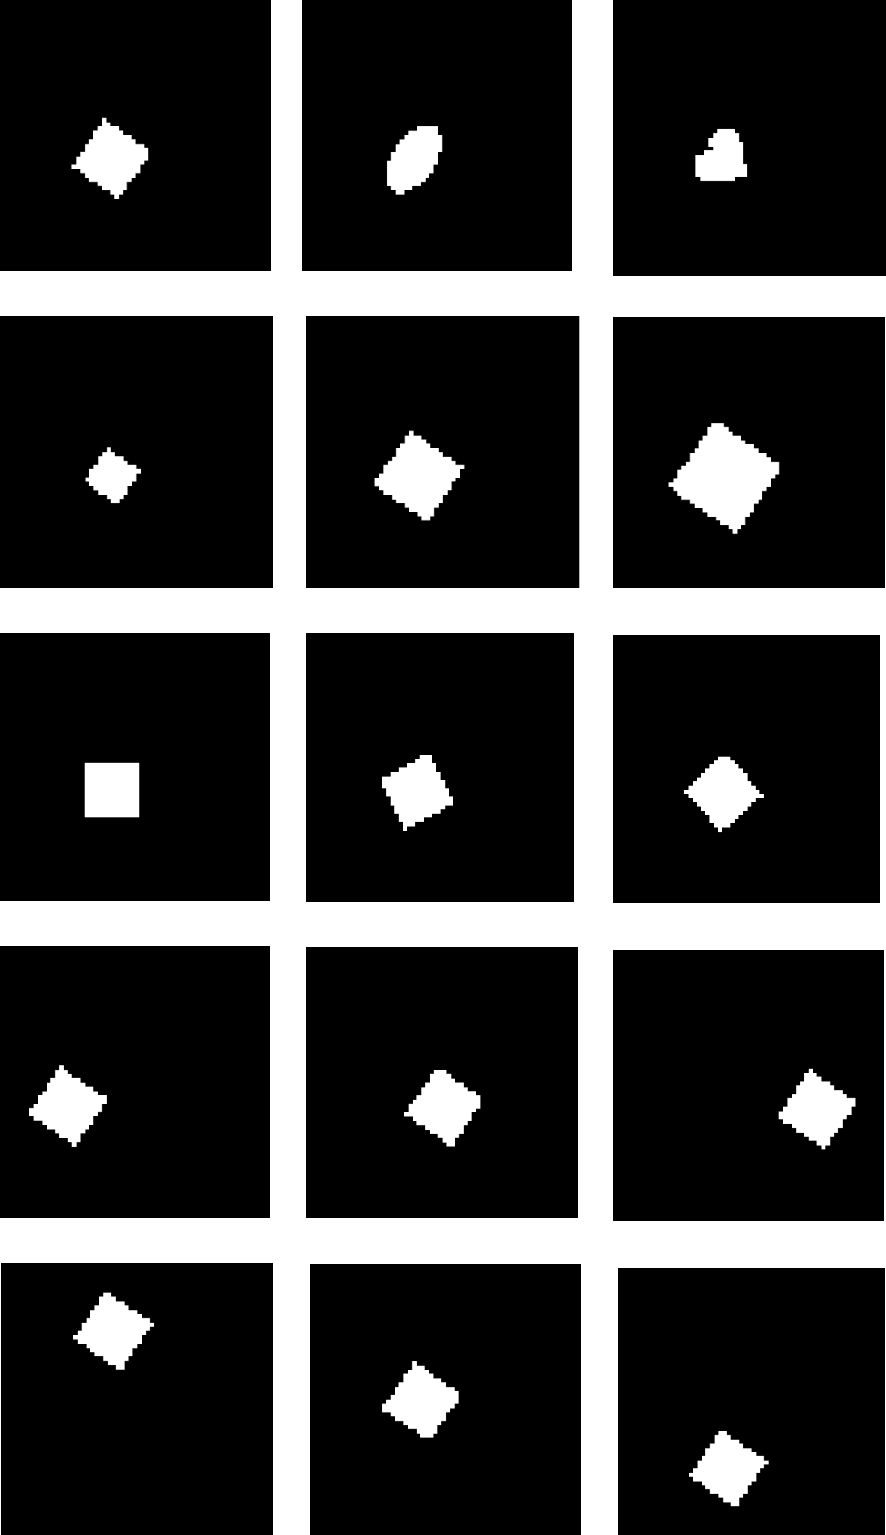
\includegraphics[width=\linewidth]{dsprites}
\end{figure}
\end{column}
\begin{column}{0.65\textwidth}
\begin{itemize}\itemsep=26pt
\item Shape: square, ellipse, heart{\color{red}{(discrete)}}
\item Scale: 6 values linearly spaced in $[0.5, 1]$
\item Orientation: 40 values in $[0, 2\pi]$
\item Position X: 32 values in $[0, 1]$
\item Position Y: 32 values in $[0, 1]$

\end{itemize}
\end{column}
\end{columns}

\end{frame}

\begin{frame}
\frametitle{Quantitative results on dSprites}
\begin{columns}
\begin{column}{0.5\textwidth}
\begin{table}[htbp]
\centering
\fontsize{9pt}{9.5pt}\selectfont
\begin{tabular}{rc rr}
\addlinespace[-\aboverulesep]
\toprule
\multicolumn{1}{c}{Method}&m&\multicolumn{1}{c}{Mean (std)}&\multicolumn{1}{c}{Best}\\
\toprule
$\beta$ VAE\\($\beta=10.0$)& 5 & 70.11 (7.54)&84.62\\
($\beta=4.0$)& 10 &74.41 (7.68)&88.38\\
\midrule
FactorVAE& 5  &81.09 (2.63)&85.12\\
        & 10 &82.15 (0.88)&88.25\\
\midrule
CascadeVAE-C\\($\beta_l=0.7$)& 5  &81.69 (3.14)&88.38\\
    ($\beta_l=1.0$)& 10 &81.74 (2.97)&87.38\\
\midrule
\midrule
JointVAE & 6 &  74.51 (5.17)&91.75\\
        & 4 &  73.06 (2.18)&75.38\\
\midrule
CascadeVAE\\($\beta_l=1.0$)& 6 &90.49 (5.28)&\textbf{99.50}\\
($\beta_l=2.0$)& 4 &\textbf{91.34 (7.36)}&98.62\\
\bottomrule
\end{tabular}
\end{table}
\end{column}
\begin{column}{0.35\textwidth}
\begin{itemize}\itemsep=12pt
\item {\color{blue}{Disentanglement score}} is obtained from 10 different random seed each with the best hyperparameters. 
\item $m$ is the number of continous latent dimensions.
\end{itemize}
\end{column}
\end{columns}
\end{frame}


\begin{frame}
\frametitle{Quantitative results on dSprites}
\begin{columns}
\begin{column}{0.5\textwidth}
\begin{table}[htbp]
\fontsize{9pt}{9.5pt}\selectfont
\centering
\begin{tabular}{rc ll}
\addlinespace[-\aboverulesep]
\toprule
\multicolumn{1}{c}{Method}&m&\multicolumn{1}{c}{Mean (std)}&\multicolumn{1}{c}{Best}\\
\toprule
JointVAE & 6&44.79 (3.88) &53.14\\
        &  4&43.99 (3.94) &54.11\\
\midrule
CascadeVAE &6&\textbf{78.84 (15.65)}& \textbf{99.66}\\
                &4&76.00 (22.16)& 98.72\\
\bottomrule
\end{tabular}
\end{table}
\end{column}
\begin{column}{0.4\textwidth}
\begin{itemize}\itemsep=12pt
\item {\color{blue}{Unsupervised classification accuracy}} when size of discrete variable is 3.
\item Unsupervised classification accuray for random chance is $33.33$.
\end{itemize}

\end{column}
\end{columns}
\end{frame}


%%\begin{frame}
%%\frametitle{Quantitative results on dSprites}
%%\begin{figure}[]
%%\centering
%%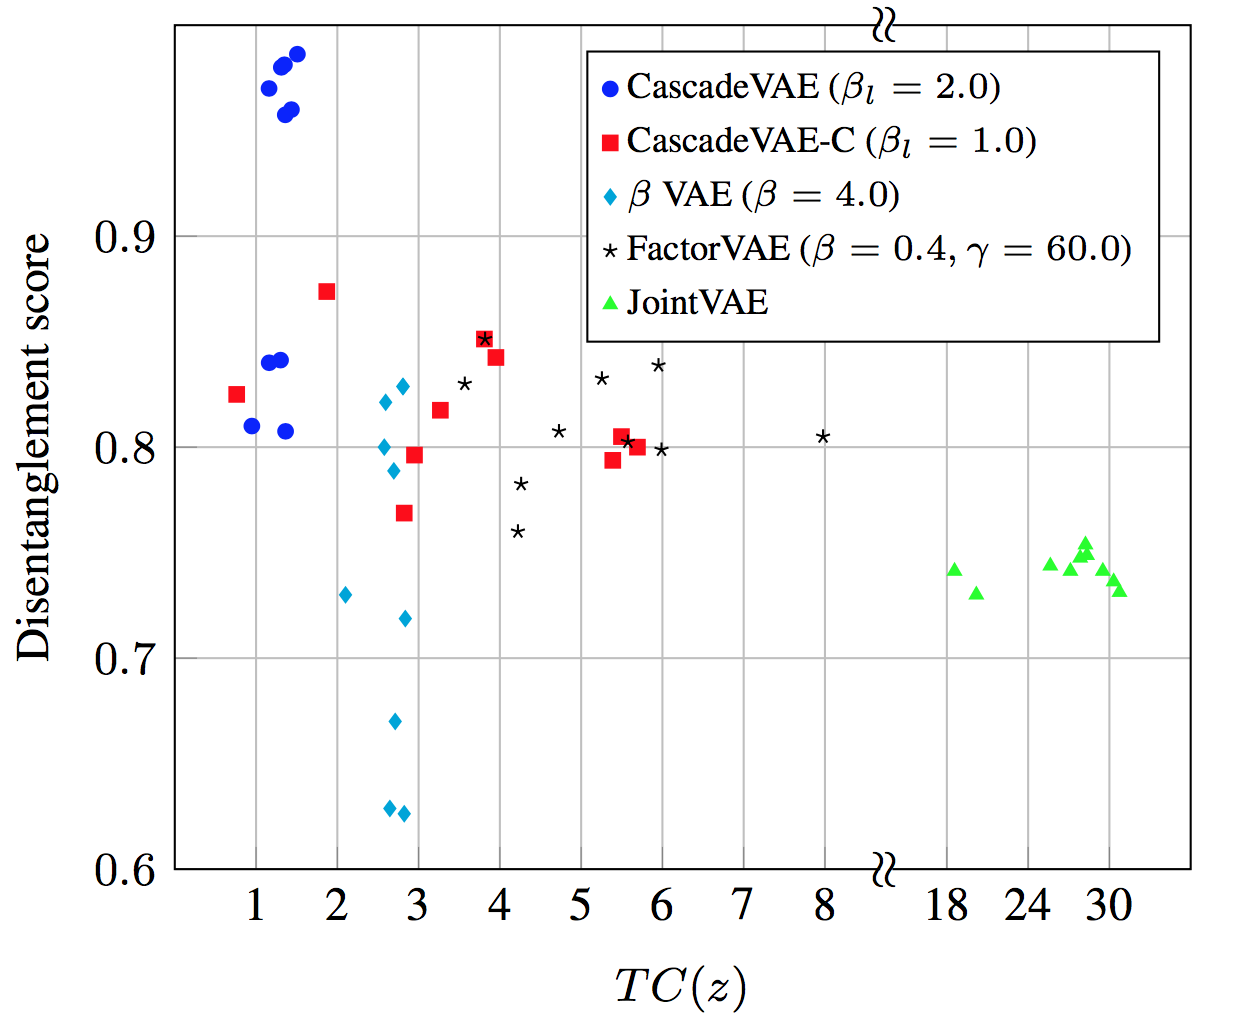
\includegraphics[width=0.65\linewidth]{tc_score.png}
%%\end{figure}
%%\end{frame}

%%\begin{frame}
%%\frametitle{Qualitative results on dSprites}
%%\begin{figure}
%%\centering
%%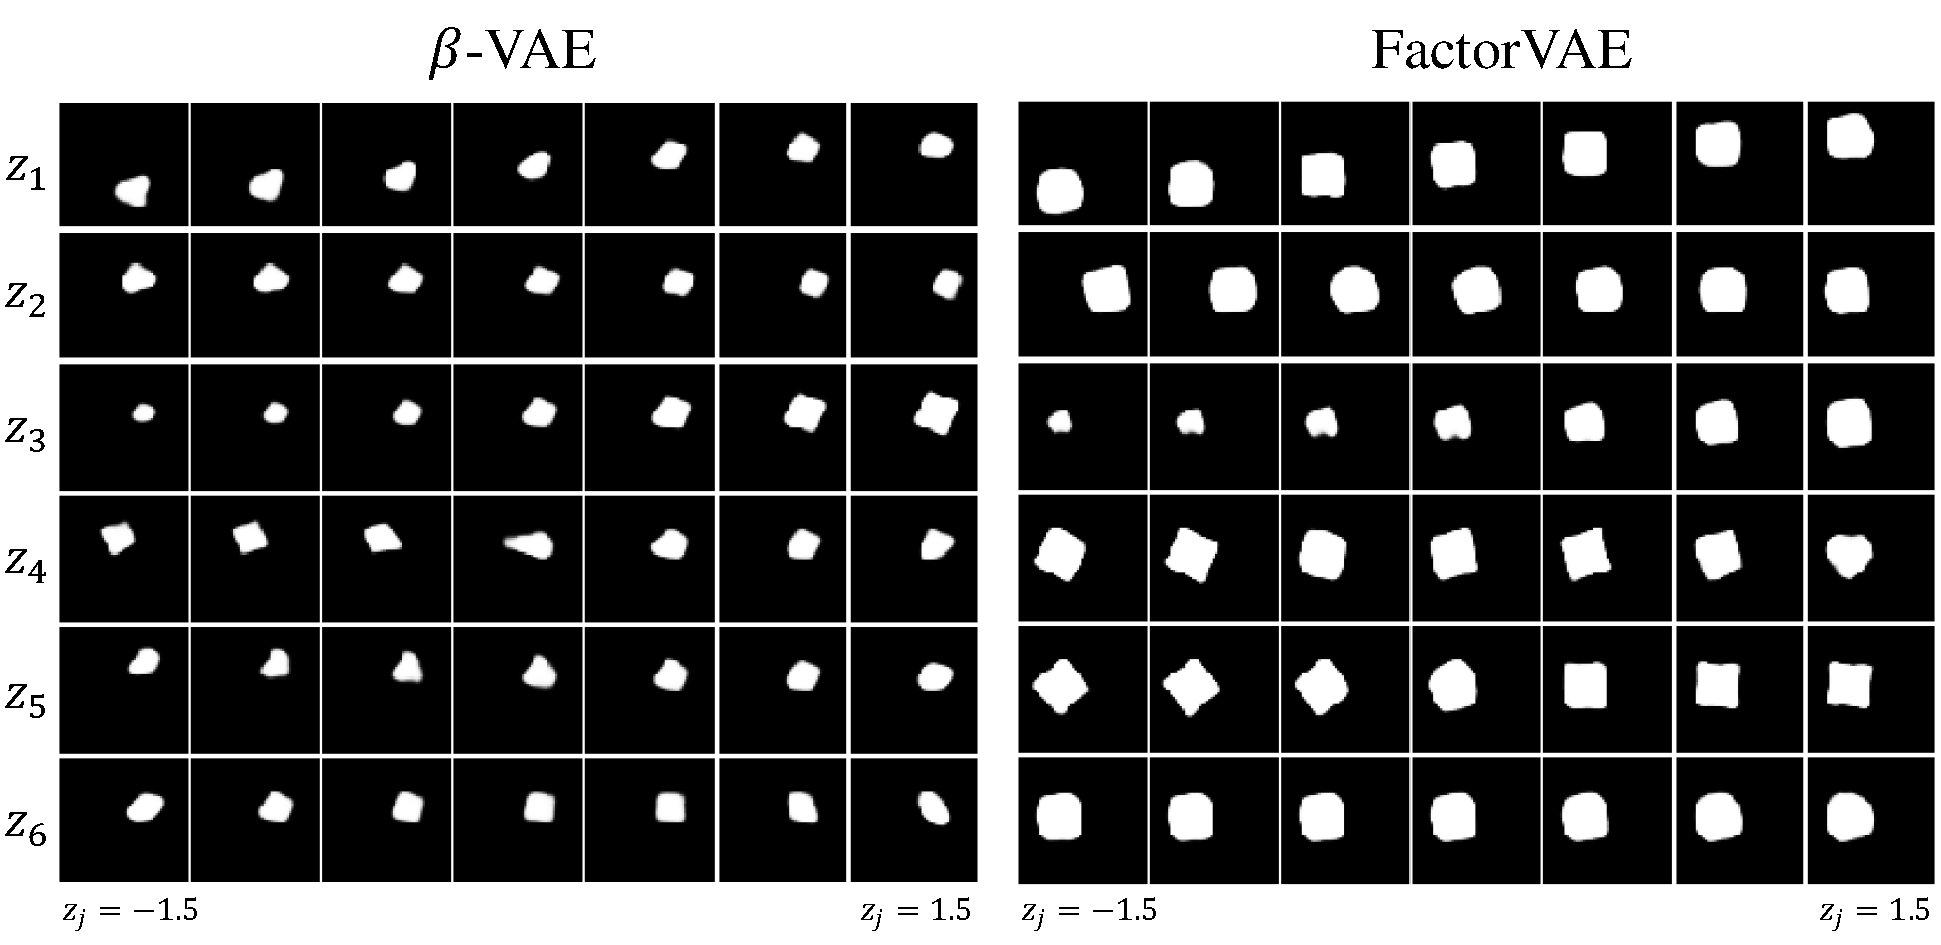
\includegraphics[width=0.9\textwidth,center]{dsprites_beta_factor}
%%\end{figure}
%%\end{frame}

\begin{frame}
\frametitle{DSprites gif animation}
\begin{itemize}\itemsep=8pt
\item $\beta$-VAE\\
$\mathbf{\qquad\quad z_1\qquad\qquad~z_2\qquad\qquad~z_3\qquad\qquad~z_4\qquad\qquad~~z_5}$
\vspace{-0.6em}
\begin{figure}
\centering
\only<1>{
\includegraphics[width=0.9\textwidth,center]{vae_gif/vae-0.png}}%
\only<2>{
\includegraphics[width=0.9\textwidth,center]{vae_gif/vae-5.png}}%
\only<3>{
\includegraphics[width=0.9\textwidth,center]{vae_gif/vae-10.png}}%
\only<4>{
\includegraphics[width=0.9\textwidth,center]{vae_gif/vae-15.png}}%
\only<5>{
\includegraphics[width=0.9\textwidth,center]{vae_gif/vae-20.png}}%
\only<6>{
\includegraphics[width=0.9\textwidth,center]{vae_gif/vae-25.png}}%
\only<7>{
\includegraphics[width=0.9\textwidth,center]{vae_gif/vae-30.png}}%
\only<8>{
\includegraphics[width=0.9\textwidth,center]{vae_gif/vae-35.png}}%
\only<9>{
\includegraphics[width=0.9\textwidth,center]{vae_gif/vae-40.png}}%
\only<10>{
\includegraphics[width=0.9\textwidth,center]{vae_gif/vae-45.png}}
\end{figure}
\item FactorVAE\\
$\mathbf{\qquad\quad z_1\qquad\qquad~z_2\qquad\qquad~z_3\qquad\qquad~z_4\qquad\qquad~~z_5}$
\vspace{-0.6em}
\begin{figure}
\only<1>{
\includegraphics[width=0.9\textwidth,center]{factor_gif/factor-0.png}}%
\only<2>{
\includegraphics[width=0.9\textwidth,center]{factor_gif/factor-5.png}}%
\only<3>{
\includegraphics[width=0.9\textwidth,center]{factor_gif/factor-10.png}}%
\only<4>{
\includegraphics[width=0.9\textwidth,center]{factor_gif/factor-15.png}}%
\only<5>{
\includegraphics[width=0.9\textwidth,center]{factor_gif/factor-20.png}}%
\only<6>{
\includegraphics[width=0.9\textwidth,center]{factor_gif/factor-25.png}}%
\only<7>{
\includegraphics[width=0.9\textwidth,center]{factor_gif/factor-30.png}}%
\only<8>{
\includegraphics[width=0.9\textwidth,center]{factor_gif/factor-35.png}}%
\only<9>{
\includegraphics[width=0.9\textwidth,center]{factor_gif/factor-40.png}}%
\only<10>{
\includegraphics[width=0.9\textwidth,center]{factor_gif/factor-45.png}}
\end{figure}
\end{itemize}
\end{frame}

\begin{frame}
\frametitle{DSprites gif animation}
\begin{itemize}\itemsep=8pt
\item JointVAE\\
\end{itemize}
\begin{columns}
\begin{column}{0.03\textwidth}
\vspace{0.5em}\\
$\mathbf{d=[1 0 0]}$\\\vspace{3em}
$\mathbf{d=[0 1 0]}$\\\vspace{3em}
$\mathbf{d=[0 0 1]}$
\end{column}
\begin{column}{0.98\textwidth}
$\mathbf{\qquad\quad~~z_1\qquad\quad~z_2\qquad\quad~ z_3\qquad\quad~z_4\qquad\quad~z_5\qquad\quad~z_6}$
\vspace{-1em}
\begin{figure}
\centering
\only<1>{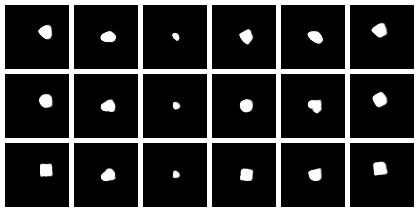
\includegraphics[width=0.9\textwidth,center]{joint_gif/jointvae-0.png}}%
\only<2>{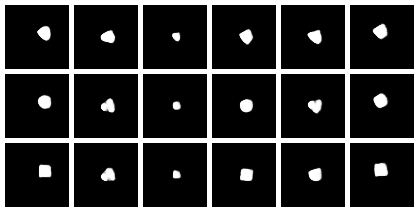
\includegraphics[width=0.9\textwidth,center]{joint_gif/jointvae-5.png}}%
\only<3>{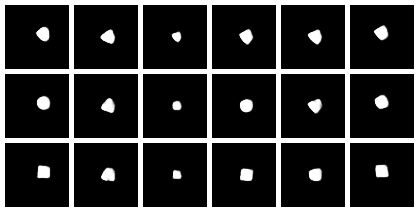
\includegraphics[width=0.9\textwidth,center]{joint_gif/jointvae-10.png}}%
\only<4>{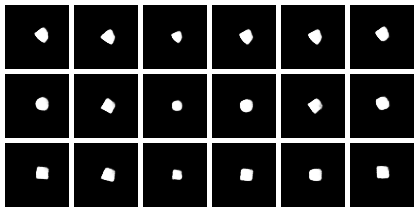
\includegraphics[width=0.9\textwidth,center]{joint_gif/jointvae-15.png}}%
\only<5>{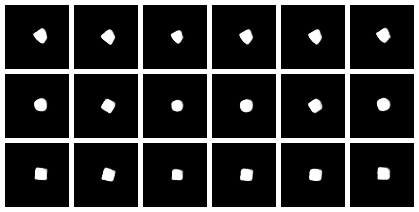
\includegraphics[width=0.9\textwidth,center]{joint_gif/jointvae-20.png}}%
\only<6>{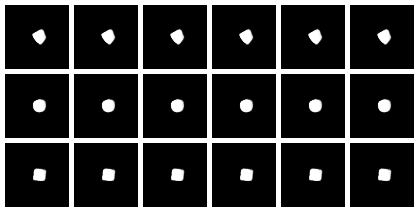
\includegraphics[width=0.9\textwidth,center]{joint_gif/jointvae-25.png}}%
\only<7>{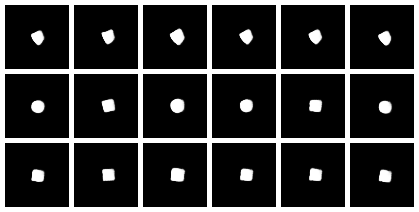
\includegraphics[width=0.9\textwidth,center]{joint_gif/jointvae-30.png}}%
\only<8>{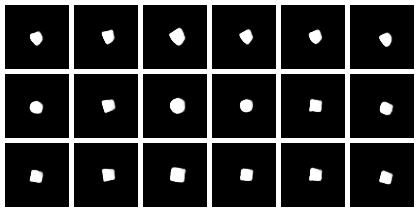
\includegraphics[width=0.9\textwidth,center]{joint_gif/jointvae-35.png}}%
\only<9>{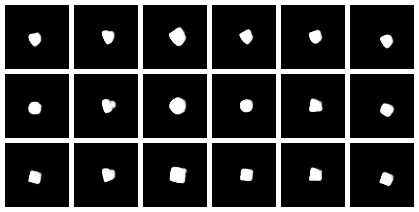
\includegraphics[width=0.9\textwidth,center]{joint_gif/jointvae-40.png}}%
\only<10>{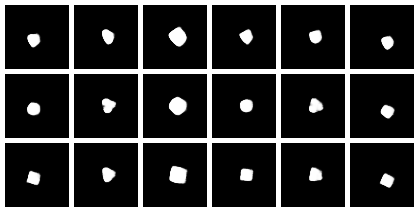
\includegraphics[width=0.9\textwidth,center]{joint_gif/jointvae-45.png}}
\end{figure}

\end{column}
\end{columns}

\end{frame}

\begin{frame}
\frametitle{DSprites gif animation}
\begin{itemize}\itemsep=8pt
\item CascadeVAE\\
\end{itemize}
\begin{columns}
\begin{column}{0.03\textwidth}
\vspace{0.5em}\\
$\mathbf{d=[1 0 0]}$\\\vspace{3em}
$\mathbf{d=[0 1 0]}$\\\vspace{3em}
$\mathbf{d=[0 0 1]}$
\end{column}
\begin{column}{0.98\textwidth}
$\mathbf{\qquad\quad~~z_1\qquad\quad~z_2\qquad\quad~ z_3\qquad\quad~z_4\qquad\quad~z_5\qquad\quad~z_6}$
\vspace{-1em}
\begin{figure}
\centering
\only<1>{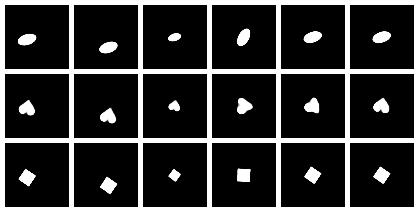
\includegraphics[width=0.9\textwidth,center]{cascade_gif/cascade-0.png}}%
\only<2>{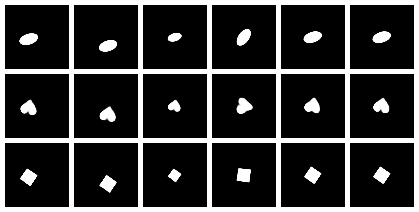
\includegraphics[width=0.9\textwidth,center]{cascade_gif/cascade-5.png}}%
\only<3>{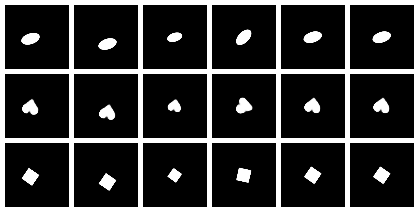
\includegraphics[width=0.9\textwidth,center]{cascade_gif/cascade-10.png}}%
\only<4>{\includegraphics[width=0.9\textwidth,center]{cascade_gif/cascade-15.png}}%
\only<5>{\includegraphics[width=0.9\textwidth,center]{cascade_gif/cascade-20.png}}%
\only<6>{\includegraphics[width=0.9\textwidth,center]{cascade_gif/cascade-25.png}}%
\only<7>{\includegraphics[width=0.9\textwidth,center]{cascade_gif/cascade-30.png}}%
\only<8>{\includegraphics[width=0.9\textwidth,center]{cascade_gif/cascade-35.png}}%
\only<9>{\includegraphics[width=0.9\textwidth,center]{cascade_gif/cascade-40.png}}%
\only<10>{\includegraphics[width=0.9\textwidth,center]{cascade_gif/cascade-45.png}}
\end{figure}
\end{column}
\end{columns}
\end{frame}


\begin{frame}
\frametitle{Quantitative results on MNIST}
\begin{columns}
\begin{column}{0.5\textwidth}
\begin{table}[htbp]
\centering
\fontsize{9pt}{9.5pt}\selectfont
\begin{tabular}{rc rr}
\addlinespace[-\aboverulesep]
\toprule
\multicolumn{1}{c}{Method}&m& \multicolumn{1}{c}{Mean (std)}&\multicolumn{1}{c}{Best}\\
\toprule
JointVAE & 10&68.57 (9.19) &82.30\\
        &  4&78.33 (7.18) &92.81\\
\midrule
CascadeVAE &10&81.41 (9.54)& \textbf{97.31}\\
           & 4&\textbf{84.19 (5.02)}& 96.39\\
\bottomrule
\end{tabular}
\end{table}
\end{column}
\begin{column}{0.4\textwidth}
\begin{itemize}\itemsep=12pt
\item {\color{blue}{Unsupervised classification accuracy}} when size of discrete variable is 10.
\item Unsupervised classification accuray for random chance is $10.00$.
\end{itemize}

\end{column}
\end{columns}
\end{frame}


\begin{frame}
\frametitle{Qualitative results on MNIST}
\begin{figure}[bp]
\centering
\begin{subfigure}[t]{0.48\linewidth}
\centering
\includegraphics[width=0.8\linewidth]{mnist_slant.png}
\caption{Angle}
\end{subfigure}\hspace{0.005\linewidth}
\begin{subfigure}[t]{0.48\linewidth}
\centering
\includegraphics[width=0.8\linewidth]{mnist_width.png}
\caption{Width}
\end{subfigure}\hspace{0.005\linewidth}
\begin{subfigure}[t]{0.48\linewidth}
\centering
\includegraphics[width=0.8\linewidth]{mnist_style.png}
\caption{Stroke}
\end{subfigure}\hspace{0.005\linewidth}
\begin{subfigure}[t]{0.48\linewidth}
\centering
\includegraphics[width=0.8\linewidth]{mnist_thickness.png}
\caption{Thickness}
\end{subfigure}
\caption{ Latent traversals on MNIST. Images in a row has the same latent variables except the traversed variable.}
\end{figure}
\end{frame}

\begin{frame}
\frametitle{Qualitative results on MNIST}
\begin{figure}[bp]
\centering
\includegraphics[width=0.8\linewidth]{mnist_digit.png}
\caption{MNIST discrete latent space traversal. Images in a row has the same latent variables except discrete variable.}
\end{figure}
\end{frame}

\begin{frame}
\frametitle{Qualitative results on Chairs}
\begin{figure}[htbp]
\centering
\includegraphics[width=\linewidth]{chairs}
\caption{Latent space traversal on chairs dataset. The last row shows the latent traversal of the discrete factor of dimension 3 with the period of 3.}
\label{fig:chairs_latent_traversal}
\end{figure}
\end{frame}

\begin{frame}
\frametitle{Conclusion}
\begin{itemize}\itemsep=12pt
\item We first propose an efficient procedure for implicitly penalizing the total correlation by controlling the information flow on each variables without using extra discriminator networks or sampling procedures.
\item We show a method for jointly learning discrete and continuous latent variables in an alternating maximization framework where we alternate between {\color{blue}{finding the most likely discrete configurations based on the continuous latent variables}}, and {\color{blue}{updating the inference parameters based on the discrete variables}}. 
\end{itemize}
\end{frame}

\begin{frame}
\frametitle{Conclusion}
\begin{itemize}
\item Our ablation study shows that information cascading and alternating maximization of discrete and continuous variables, provide complementary benefits and leads to the state of the art performance in 1) disentanglement score, and 2) classification accuracy score from the discrete inference network, compared to a number of recently proposed methods.
\end{itemize}
\end{frame}


\end{document}




